\section{Model Description}

\subsection{Introduction}

The hinged rigid body class is an instantiation of the state effector abstract class. The state effector abstract class is a base class for modules that have dynamic states or degrees of freedom with respect to the rigid body hub. Examples of these would be reaction wheels, variable speed control moment gyroscopes, fuel slosh particles, etc. Since the state effectors are attached to the hub, the state effectors are directly affecting the hub as well as the hub is back affecting the state effectors.

Specifically, a hinged rigid body state effector is a rigid body that has a diagonal inertia with respect to its $\mathcal{S}_i$ frame as seen in Figure~\ref{fig:FlexFigure}. It is attached to the hub through a hinge with a linear torsional spring and linear damping term.  An optional motor torque command can be used to actuate the panel.  The dynamics of this multi-body problem have been derived and can be seen in Reference~\citenum{Allard2016rz}. The derivation is general for $N$ number of panels attached to the hub but does not allow for multiple interconnected panels. 

\begin{figure}[htbp]
	\centerline{
		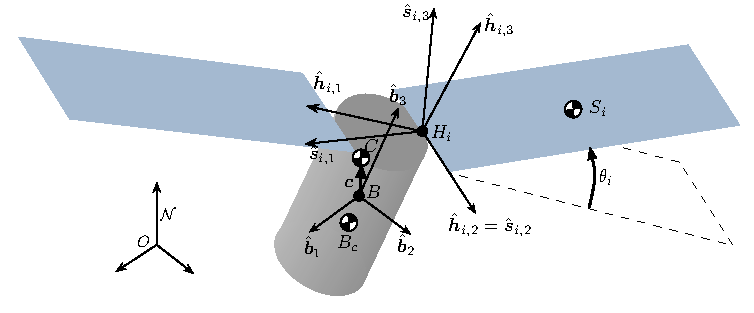
\includegraphics[width=0.8\textwidth]{Figures/Fig4_4_2}}
	\caption{Hinged rigid body frame and variable definitions}
	\label{fig:FlexFigure}
\end{figure}

\subsection{Equations of Motion}

The following equations of motion (EOMs) are pulled from Reference~\citenum{Allard2016rz} for convenience. Equation~\eqref{eq:Rbddot3} is the spacecraft translational EOM, Equation~\eqref{eq:Final6} is the spacecraft rotational EOM, and Equation~\eqref{eq:solar_panel_final3} is the hinged rigid body rotational EOM. These are the coupled nonlinear EOMs that need to be integrated in the simulation. 

\begin{multline}
m_{\text{sc}} \ddot{\bm r}_{B/N}-m_{\text{sc}} [\tilde{\bm{c}}]\dot{\bm\omega}_{\cal B/N}+\sum_{i}^{N}m_{\text{sp}_i} d_i  \bm{\hat{s}}_{i,3}\ddot{\theta}_i = \bm F_{\textnormal{ext}} - 2 m_{\text{sc}} [\tilde{\bm\omega}_{\cal B/N}]\bm{c}'\\
-m_{\text{sc}} [\tilde{\bm\omega}_{\cal B/N}][\tilde{\bm\omega}_{\cal B/N}]\bm{c}-\sum_{i}^{N}m_{\text{sp}_i}d_i\dot{\theta}_i^2 \bm{\hat{s}}_{i,1}
\label{eq:Rbddot3}
\end{multline}

\begin{multline}
	m_{\text{sc}}[\tilde{\bm{c}}]\ddot{\bm r}_{B/N}+[I_{\text{sc},B}] \dot{\bm\omega}_{\cal B/N} +\sum\limits_{i}^{N}\biggl\lbrace I_{s_i,2}\bm{\hat{h}}_{i,2}+m_{\text{sp}_i}d_i [\tilde{\bm{r}}_{S_i/B}] \bm{\hat{s}}_{i,3}\biggr\rbrace\ddot{\theta}_i = \\
	-[\bm{\tilde{\omega}}_{\cal B/N}] [I_{\text{sc},B}] \bm\omega_{\cal B/N} 
	- [I'_{\text{sc},B}] \bm\omega_{\cal B/N} - \sum\limits_{i}^{N}\biggl\lbrace\dot{\theta}_i [\bm{\tilde{\omega}}_{\cal B/N}] \left(I_{s_i,2} \bm{\hat{h}}_{i,2}+m_{\text{sp}_i} d_i [\tilde{\bm{r}}_{S_i/B}] \hat{\bm s}_{i,3}\right)\\ +m_{\text{sp}_i}d_i\dot{\theta}_i^2[\tilde{\bm{r}}_{S_i/B}] \bm{\hat{s}}_{i,1} \biggr\rbrace + \bm{L}_B
	\label{eq:Final6}
\end{multline}

\begin{multline}
m_{\text{sp}_i} d_i \hat{\bm s}_{i,3}^{T} \ddot{\bm r}_{B/N}+ \biggl[\left(I_{s_{i,2}} + m_{\text{sp}_i}d_i^{2}\right) \hat{\bm s}_{i,2}^{T}-m_{\text{sp}_i} d_i \hat{\bm s}_{i,3}^{T} [\tilde{\bm r}_{H_i/B}]\biggr] \dot{\bm\omega}_{\cal B/N} \\
+ \left( I_{s_{i,2}} + m_{\text{sp}_i} d_i^{2} \right) \ddot \theta_i 
= u_i - k_i \theta_i - c_i \dot\theta_i + \hat{\bm s}_{i,2}^T \bm \tau_{\text{ext},H_i} + \left( I_{s_{i,3}} - I_{s_{i,1}} + m_{\text{sp}_i}d_i^{2}\right) \omega_{s_{i,3}} \omega_{s_{i,1}}\\
- m_{\text{sp}_i} d_i \hat{\bm s}_{i,3}^{T} [\tilde{\bm\omega}_{\cal B/N}][\tilde{\bm\omega}_{\cal B/N}] \bm r_{H_i/B} 
\label{eq:solar_panel_final3}
\end{multline}
where $u_i$ is the optional motor torque.

\subsection{Back Substitution Method}

In order to integrate the EOMs in a modular fashion, a back substitution method was developed and can be seen in Reference~\cite{Allard2016rz}. The hinged rigid body model must adhere to this analytical form, and the details are briefly summarized in the equations following. First the hinged rigid body EOM is substituted into the translational EOM and rearranged:
\begin{multline}
\Big(m_{\text{sc}} [I_{3\times3}] +\sum_{i=1}^{N}m_{\text{sp}_i}d_i \bm{\hat{s}}_{i,3} \bm a_{\theta_i}^T\Big)\ddot{\bm r}_{B/N}+\Big(-m_{\text{sc}} [\tilde{\bm{c}}] +\sum_{i=1}^{N}m_{\text{sp}_i}d_i \bm{\hat{s}}_{i,3} \bm b_{\theta_i}^T\Big) \dot{\bm\omega}_{\cal B/N} \\
= m_{\text{sc}} \ddot{\bm r}_{C/N} 	- 2 m_{\text{sc}} [\tilde{\bm\omega}_{\cal B/N}] \bm c'
-m_{\text{sc}} [\tilde{\bm\omega}_{\cal B/N}][\tilde{\bm\omega}_{\cal B/N}]\bm{c}
-\sum_{i=1}^{N}\Big(m_{\text{sp}_i}d_i \dot{\theta}_i^2 \bm{\hat{s}}_{i,1}+m_{\text{sp}_i}d_i c_{\theta_i} \bm{\hat{s}}_{i,3} \Big)
\label{eq:Rbddot8}
\end{multline}

Following the same pattern for the hub rotational EOM, Eq.~\eqref{eq:Final6}, yields:
\begin{multline}
\Big[m_{\text{sc}}[\tilde{\bm{c}}] +\sum\limits_{i=1}^{N}\big( I_{s_{i,2}}\bm{\hat{s}}_{i,2}+m_{\text{sp}_i}d_i [\tilde{\bm{r}}_{S_{c,i}/B}] \bm{\hat{s}}_{i,3}\big)\bm a_{\theta_i}^T \Big]\ddot{\bm r}_{B/N}\\
+\Big[[I_{\text{sc},B}]+\sum\limits_{i=1}^{N}\big( I_{s_{i,2}}\bm{\hat{s}}_{i,2}+m_{\text{sp}_i}d_i [\tilde{\bm{r}}_{S_{c,i}/B}] \bm{\hat{s}}_{i,3}\big) \bm b_{\theta_i}^T\Big] \dot{\bm\omega}_{\cal B/N}
= 
-[\bm{\tilde{\omega}}_{\cal B/N}] [I_{\text{sc},B}] \bm\omega_{\cal B/N} 
- [I'_{\text{sc},B}] \bm\omega_{\cal B/N} \\
-\sum\limits_{i=1}^{N}\biggl\lbrace\big(\dot{\theta}_i [\bm{\tilde{\omega}}_{\cal B/N}] +c_{\theta_i} [I_{3\times3}]\big) \left(I_{s_{i,2}} \bm{\hat{s}}_{i,2}+m_{\text{sp}_i} d_i [\tilde{\bm{r}}_{S_{c,i}/B}] \hat{\bm s}_{i,3}\right) +m_{\text{sp}_i}d_i\dot{\theta}_i^2[\tilde{\bm{r}}_{S_{c,i}/B}] \bm{\hat{s}}_{i,1} \biggr\rbrace + \bm{L}_B
\label{eq:Final9}
\end{multline}	

With the following definitions:

\begin{subequations}
	\begin{align}
	\bm a_{\theta_i} &= - \frac{m_{\text{sp}_i} d_i}{\left( I_{s_{i,2}} + m_{\text{sp}_i} d_i^{2} \right)} \hat{\bm s}_{i,3}
	\label{eq:solar_panel_final11}
	\\
	\bm b_{\theta_i} &= -\frac{1}{\left( I_{s_{i,2}} + m_{\text{sp}_i} d_i^{2} \right)} \bigg[\left(I_{s_{i,2}} + m_{\text{sp}_i}d_i^{2}\right) \hat{\bm s}_{i,2}+m_{\text{sp}_i} d_i [\tilde{\bm r}_{H_i/B}] \hat{\bm s}_{i,3}\bigg]
	\\
	\begin{split}
	c_{\theta_i} &= \frac{1}{\left( I_{s_{i,2}} + m_{\text{sp}_i} d_i^{2} \right)} \Big(u_i - k_i \theta_i - c_i \dot\theta_i + \hat{\bm s}_{i,2} \cdot \bm \tau_{\text{ext},H_i} + \left( I_{s_{i,3}} - I_{s_{i,1}} + m_{\text{sp}_i}d_i^{2}\right) \omega_{s_{i,3}} \omega_{s_{i,1}} \\
	&- m_{\text{sp}_i} d_i \hat{\bm s}_{i,3}^{T} [\tilde{\bm\omega}_{\cal B/N}][\tilde{\bm\omega}_{\cal B/N}] \bm r_{H_i/B}\Big)
	\label{eq:solar_panel_final6}
	\end{split}
	\end{align}
\end{subequations}
In Eq.~\eqref{eq:solar_panel_final6} the variable $u_i$ is the motor torque acting on the $i^{\text{th}}$ panel.

The equations can now be organized into the following matrix representation:
\begin{equation}
\begin{bmatrix}
[A] & [B]\\
[C] & [D]
\end{bmatrix} \begin{bmatrix}
\ddot{\bm r}_{B/N}\\
\dot{\bm\omega}_{\cal B/N}
\end{bmatrix} = \begin{bmatrix}
\bm v_{\text{trans}}\\
\bm v_{\text{rot}}
\end{bmatrix}
\label{eq:backSub}
\end{equation}

Finally, the hinged rigid body model must make ``contributions" to the matrices defined in Equations~\eqref{eq:backSub}. These contributions are defined in the following equations: 

\begin{align}
[A_{\textnormal{contr}}] &= m_{\text{sp}_i}d_i \bm{\hat{s}}_{i,3} \bm a_{\theta_i}^T
\\
[B_{\textnormal{contr}}] &= m_{\text{sp}_i}d_i \bm{\hat{s}}_{i,3} \bm b_{\theta_i}^T 
\\
[C_{\textnormal{contr}}] &= \big( I_{s_{i,2}}\bm{\hat{s}}_{i,2}+m_{\text{sp}_i}d_i [\tilde{\bm{r}}_{S_{c,i}/B}] \bm{\hat{s}}_{i,3}\big)\bm a_{\theta_i}^T
\\
[D_{\textnormal{contr}}] &= \big( I_{s_{i,2}}\bm{\hat{s}}_{i,2}+m_{\text{sp}_i}d_i [\tilde{\bm{r}}_{S_{c,i}/B}] \bm{\hat{s}}_{i,3}\big) \bm b_{\theta_i}^T
\\
\bm v_{\text{trans,contr}} &= -\Big(m_{\text{sp}_i}d_i \dot{\theta}_i^2 \bm{\hat{s}}_{i,1}+m_{\text{sp}_i}d_i c_{\theta_i} \bm{\hat{s}}_{i,3} \Big)
\\
\bm v_{\text{rot,contr}} &= -\biggl\lbrace\big(\dot{\theta}_i [\bm{\tilde{\omega}}_{\cal B/N}] +c_{\theta_i} [I_{3\times3}]\big) \left(I_{s_{i,2}} \bm{\hat{s}}_{i,2}+m_{\text{sp}_i} d_i [\tilde{\bm{r}}_{S_{c,i}/B}] \hat{\bm s}_{i,3}\right) +m_{\text{sp}_i}d_i\dot{\theta}_i^2[\tilde{\bm{r}}_{S_{c,i}/B}] \bm{\hat{s}}_{i,1} \biggr\rbrace 
\end{align}

The final equation that is needed is:

\begin{equation}
\ddot \theta_i = \bm a_{\theta_i}^T \ddot{\bm r}_{B/N} + \bm b_{\theta_i}^T \dot{\bm\omega}_{\cal B/N} + c_{\theta_i}
\label{eq:solar_panel_final5}
\end{equation}



\subsection{Panel State Configuration Log Message Information}
The panel provides an output message {\tt hingedRigidBodyConfigLogOutMsgName} of type {\tt SCStatesMsg}.  This message contains the panel frame $S_i$ position and attitude states.  As this is a regular spacecraft state message, this output message can be piped to other modules such as the coarse sun sensor or solar panel power module spacecraft state input message.  This allows the CSS or solar power evaluation to be performed relative to the time-varying panel configuration.

The configuration log records the following 4 message variables: {\tt r\_BN\_N}, {\tt r\_BN\_N}, {\tt sigma\_BN} and {\tt omega\_BN\_B}.  These states are evaluated using:
\begin{align}
	\bm r_{S_i/N} &= \bm r_{S_i/B} + \bm r_{B/N}
	\\
	\bm v_{S_i/N} &= \dot{\bm r}_{B/N} + d_i \dot\theta_i \hat{\bm s}_{i,3} - d_i \bm\omega_{B/N}\times \hat{\bm s}_{i,1} + \bm\omega_{B/N} \times \bm r_{H_i/B}
	\\
	\bm\sigma_{S_i/N} &=  \bm\sigma_{S_i/B} \otimes\bm\sigma_{B/N}
	\\
	\bm\omega_{S_i/N} &= \bm\omega_{B/N} + \dot\theta_i \hat{\bm s}_{i,2}
\end{align}

When storing these log state the message body frame is the hinge frame $S_i$.
